\documentclass[12pt]{article}
\usepackage{amssymb}
\usepackage{amsmath}
\usepackage{amsthm}
\usepackage{mathtools}
\usepackage{array}
\usepackage{multirow}
\usepackage{colortbl}
\usepackage[dvipsnames]{xcolor}
\usepackage{graphicx}
  \DeclareGraphicsRule{*}{mps}{*}{}
%\usepackage{bbm}
\usepackage{marvosym}
\usepackage{enumerate}
\usepackage{txfonts}
\usepackage{paralist}
\usepackage{pdfpages}
\usepackage{multicol}
\usepackage{tikz}
\usepackage{siunitx}
\usepackage[normalem]{ulem}
\everymath{\displaystyle}

\usepackage[margin=.7in]{geometry}
%\usepackage{fullpage}

\setdefaultleftmargin{0pt}{}{}{}{}{}

\newcommand{\mblank}{\rule[-1ex]{8ex}{0.4pt}}
\definecolor{lightgray}{gray}{0.7}

\newenvironment{solution}
{\color{BrickRed}\textbf{Solution.} 
}
{\ignorespacesafterend}

% Circles for Venn diagrams
\def\firstcircle{(90:1cm) circle (1.5cm)}
\def\secondcircle{(210:1cm) circle (1.5cm)}
\def\thirdcircle{(330:1cm) circle (1.5cm)}
% And here's the background rectangle
\def\universer{(-3, -2.5) rectangle (3, 2.75)}


\renewcommand{\thefootnote}{\fnsymbol{footnote}}

\hyphenpenalty=5000
\tolerance=1000
\setlength{\parindent}{0pt}

\begin{document}
\pagestyle{empty}

\begin{enumerate}


\item 
\textbf{(P5)
Consider the following theorem:} 

For all natural numbers $n$, if $n^{2}$ is even then $n$ is even. 

What follows is a supposed proof. Your job is to critique the proof by explaining what is wrong with it and by supplying a correct proof. Check it out:

    \begin{proof} Consider any $n \in \mathbb{N}$. Assume that $n^{2}$ is even. 
    
    By definition, $n^{2} = 2k$ for some $k \in \mathbb{N}$.
    
    Let's take square roots of each side giving us $\sqrt{n^{2}}=\sqrt{2k}$. 
    
    Simplifying, $n=\sqrt{2k}$.  
    
    Multiplying by $2$ top and bottom inside the square root, $n=\sqrt{\frac{2\cdot 2k}{2}}$. 
    
    So, $n=\sqrt{\frac{4\cdot k}{2}}$.  
    
    Pulling $4$ out of the square root, $n=2\cdot\sqrt{\frac{k}{2}}$.
    
    Let $m=\sqrt{\frac{k}{2}}$.
    
    Thus $n=2m$.
    
    Therefore, $n$ is an even number.
    
    So, our theorem is proved!?
    \end{proof}

\item 
\textbf{(L1, S3)} Suppose that $f$ is a function with domain $A$ and codomain $B$.

\begin{enumerate}
	\item
	Write the formal definition of $f$ being a \textbf{one-to-one} function (also called a \textbf{injective} function) using needed quantifiers and connectives.
	\item
	Assume that the domain $A$ and codomain $B$ for function $f$ are both finite sets and that $f$ is a one-to-one function. What is the necessary relationship between the cardinality of $A$ and the cardinality of $B$?  Explain.
\end{enumerate}


\item
\textbf{(L3, S4)} In analyzing relations on a set we have studied the reflexive, symmetric, and transitive properties but there are other interesting and important properties. One of them is the antisymmetric property. Here is the definition.

Given relation R on set A, R is \textbf{antisymmetric} if and only if 

		\[\forall x \in A\ \forall y \in A, (xRy \land yRx) \rightarrow x = y \]

\begin{enumerate}
    \item Write an \textbf{equivalent} definition of antisymmetric in logical symbols using the contrapositive of the original definition.
	\item Write the \textbf{negation} of this definition in logical symbols. Simplify as much as possible.
	\item Draw two directed graphs for different relations on the set A={w,x,y,z}, one that \textbf{IS} antisymmetric and one that is \textbf{NOT} antisymmetric.
\end{enumerate}

\item
\textbf{(S4)} Given a relation R on set A, here are the definitions of the symmetric and antisymmetric properties:

R is \textbf{symmetric} if and only if

        \[\forall x \in A\ \forall y \in A, xRy \rightarrow yRx \]

R is \textbf{antisymmetric} if and only if 

		\[\forall x \in A\ \forall y \in A, (xRy \land yRx) \rightarrow x = y \]

\begin{enumerate}
    \item Can a relation be neither symmetric nor antisymmetric? If yes, find an example. If no, explain why not.
    \item Can a relation be both symmetric and antisymmetric? If yes, find an example. If no, explain why not.
\end{enumerate}		

\item \textbf{(S4, S5)} Here is a relation R on set $A=\{1,2,3,4,5\}$.

 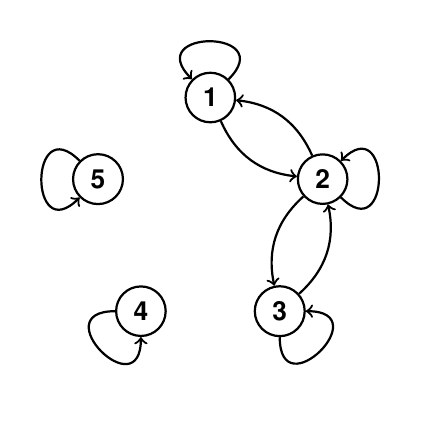
\begin{tikzpicture}[baseline, ->, thick, main node/.style={circle,draw,font=\sffamily\bfseries}]
	    \foreach \x in {1,2,3,4,5}
	        \node[main node](\x) at (162-72*\x:1.5cm) {\x};
        \draw (1) edge[loop, looseness=5] (1);
        \draw (2) to [out = -45, in = 45, looseness = 5] (2);
        \draw (3) to [out=270, in=0, looseness = 5] (3);
        \draw (4) to [out=180, in=270, looseness = 5] (4);
        \draw (5) to [out=135, in = 225, looseness = 5] (5);
        \draw (1) to [bend right] (2);
        \draw (2) to [bend right] (1);
        \draw (2) to [bend right] (3);
        \draw (3) to [bend right] (2);
        \end{tikzpicture} \hfill

\begin{enumerate}
    \item Is R reflexive? Is R symmetric? Is R transitive? (For this problem short Yes/No answers are acceptable.)
    \item Add the minimum number of directed edges necessary to make the relation an equivalence relation.
    \item For the equivalence relation in part b, identify all the equivalence classes.
\end{enumerate}

\item 
\begin{enumerate} 
\item (\textbf{C1, C3}) There are 24 students in our class, and we'd like to split everyone up into six groups of exactly 4. How many ways can we do this?\\
Carefully explain why the counting strategy you used is correct.
\item What if we're naming each of the six groups?\\
Carefully explain why the counting strategy you used is correct.
\end{enumerate}

\item (\textbf{P3}) Construct a \textbf{combinatorial} proof of the following binomial identity: 
\[\binom{n}{k} = \binom{n}{n-k}\]
(\textbf{Note:} A purely algebraic proof won't count here.)

\item (\textbf{P3}) Construct a \textbf{combinatorial} proof of the following binomial identity: 
\[\binom{n}{k} = \binom{n-1}{k-1} + \binom{n-1}{k}\]
(\textbf{Note:} A purely algebraic proof won't count here.)

\item (\textbf{P1}) Prove that an even integer minus an odd integer is an odd integer. 

(\textbf{Note:} Our usual definitions of even and odd extend to the integers pretty naturally. For instance, $-3$ is also odd, and $-4$ is also even.)

\item Suppose that $A$ and $B$ are some sets with $|A| = 10$ and $|B| = 5$.
\begin{enumerate}[(a)]
    \item (\textbf{C2}) How many functions $f:A\to B$ are surjective? (\textbf{Hint:} Whoever answers this question deserves a pie. You might think about how a function can fail to be surjective.)
    \item (\textbf{C3}) Carefully explain why the counting strategies you used in your answer are the correct ones to use.
    \item (\textbf{S3}) How many functions $g:B \to A$ are surjective? Carefully explain why your answer makes sense.
\end{enumerate}

\item (\textbf{C1, C2}) Suppose you have ten identical green balls. 

\begin{enumerate}
    \item How many ways could these balls be distributed to four people?
    \item How many ways could these balls be distributed to four people if everyone gets at least one?
    \item How many ways could these balls be distributed to four people of nobody gets more than two balls?
\end{enumerate}


\item (\textbf{C1, C3}) Our class consists of 24 individuals. 
\begin{enumerate}
    \item How many ways can an entertainment committee of three individuals be selected? Carefully explain why the counting strategy you used is correct.
    \item How many ways can an entertainment committee of three individuals be selected if one of the committee members must be the chairperson? Carefully explain why the counting strategy you used is correct.
    \item How many ways can a President, Vice President, and Treasurer be selected? Carefully explain why the counting strategy you used is correct.
 \end{enumerate}
 
\item (\textbf{S1}) Write the following sets in set-builder notation: 

\begin{enumerate}
    \item $\{1, 4, 9, 16, 25, 36, ... \}$
    \item $\{1, 4, 7, 10, 13, 16, ... \}$
\end{enumerate}


\item (\textbf{S2}) \textbf{NOTE: I think this problem is wrong!!!} Consider the following Venn diagrams and set descriptions: 

W. 
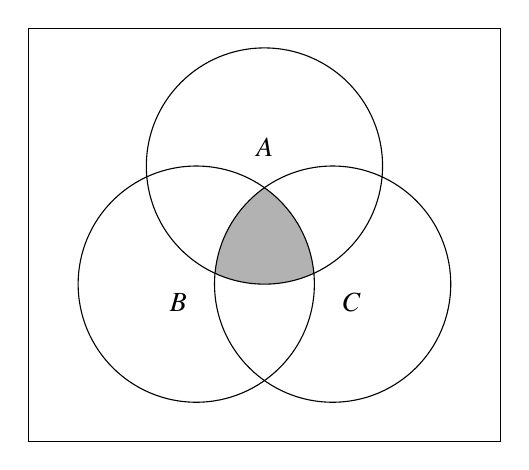
\begin{tikzpicture}
\begin{scope}
    \clip \firstcircle;
    \clip \secondcircle;
    \fill[lightgray] \thirdcircle;
\end{scope}
\draw \firstcircle node[text=black,above] {$A$};
\draw \secondcircle node [text=black,below left] {$B$};
\draw \thirdcircle node [text=black,below right] {$C$};
\draw \universer;
\end{tikzpicture}
\hfill
X. 
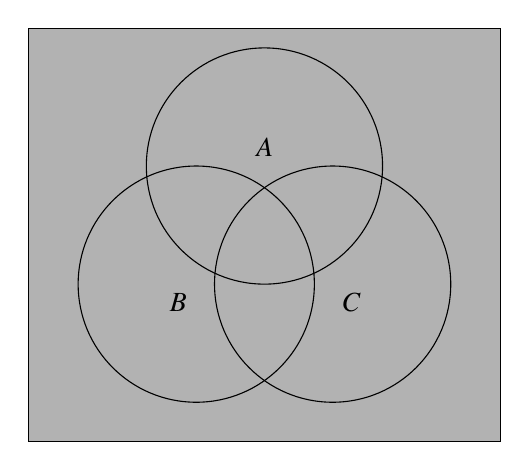
\begin{tikzpicture}
\fill[lightgray] \universer;
\draw \firstcircle node[text=black,above] {$A$};
\draw \secondcircle node [text=black,below left] {$B$};
\draw \thirdcircle node [text=black,below right] {$C$};
\draw \universer;
\end{tikzpicture}
\hfill\, % This is a ridiculous hack.

\hfill
Y.
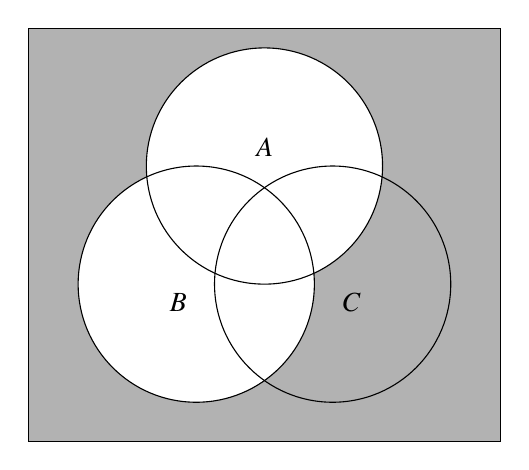
\begin{tikzpicture}
\begin{scope}[even odd rule]
    \clip \secondcircle \universer;
    \clip \firstcircle \universer;
    \fill[lightgray] \universer;
\end{scope}
\draw \firstcircle node[text=black,above] {$A$};
\draw \secondcircle node [text=black,below left] {$B$};
\draw \thirdcircle node [text=black,below right] {$C$};
\draw \universer;
\end{tikzpicture}
\hfill
Z. 
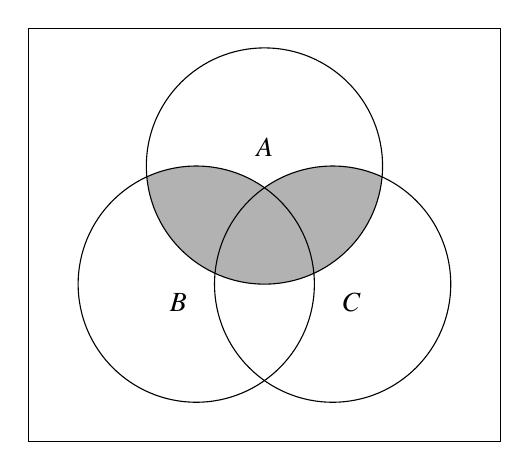
\begin{tikzpicture}
\begin{scope} % I genuinely have no idea why this works.
    \clip \secondcircle \thirdcircle;
    \fill[lightgray] \firstcircle;
\end{scope}
\draw \firstcircle node[text=black,above] {$A$};
\draw \secondcircle node [text=black,below left] {$B$};
\draw \thirdcircle node [text=black,below right] {$C$};
\draw \universer;
\end{tikzpicture}

i. $(\overline{A}) \cup (\overline{B})$
\hfill
ii. $\overline{(A \cup B)}$
\hfill
iii. $(A\cap B) \cup (A \cap C)$
\hfill
iv. $A\cap (B\cup A) \cap C$

\begin{enumerate}[(a)]
    \item Match the four Venn diagrams with the four set descriptions. Carefully explain all of your choices.
    \item Explain why it's important to carefully use parentheses when writing set descriptions.
\end{enumerate}

\item Consider the Venn diagram matching task above.
\begin{enumerate}
    \item (\textbf{C1, C3}) How many total possible ways are there to answer this question? Carefully explain why the counting strategy you used is correct.
    \item (\textbf{C2, C3}) How many answers are \textbf{completely} incorrect -- that is, contain \textbf{no} correct matches? Carefully explain your solution.
\end{enumerate}

\item (\textbf{L2}) We keep saying that the negation of an implication $(P \to Q)$ is $(P \land \lnot Q)$. 
\begin{enumerate}
    \item Write a truth table to show that this is correct.
    \item Carefully explain \textbf{why} your truth table shows that we're right.
\end{enumerate}



\item  Consider the recurrence relation $a_n = 2a_{n-1} + 8a_{n-2}$, with initial terms $a_0 = 1$ and $a_1 = 3$. 
\begin{enumerate}
    \item (\textbf{Q1}) Find the next five terms of this sequence.
    \item (\textbf{Q2}) Find a closed formula for the $n$th term of the sequence.
\end{enumerate}

\item (\textbf{Q1, Q2}) Let $a_n$ be the number of $n$-trains you can make using length-1 tiles available in 4 colors and length-2 dominos available in 5 colors.
\begin{enumerate}
    \item First, find a recurrence relation to describe the problem. Carefully explain why your recurrence relation is correct, in the context of the problem.
    \item Write out the first 6 terms of the sequence $a_1$, $a_2$, \ldots.
    \item Solve the recurrence relation to find a closed formula for $a_n$.
\end{enumerate}

\item (\textbf{P4}) Prove using mathematical induction that $1^3 + 2^3 + 3^3 + \ldots + n^3 = \left(\frac{n(n+1)}{2}\right)^2$ for all natural numbers $n \geq 1$. 

\item (\textbf{P4}) Prove using mathematical induction that every set containing $n$ elements has $2^n$ subsets for any natural number $n \geq 1$. 


\item  (\textbf{L2}) DeMorgan's Rule describes how to negate ``\textbf{and}'' statements. Use a truth table to show that  $\lnot(P \land Q)$ is logically equivalent to  $\lnot P \lor \lnot Q$.  Carefully explain \textbf{why} your truth table shows that we're right.

\item (\textbf{S2}) You are hosting a party for 50 people. As a conscientious host, you've carefully asked all of your attendees what they are allergic to: shellfish (S), peanuts (P), and/or broccoli (B). Here are the results:

\begin{tabular}{l|ccccccc}
Allergen & S  & P  & B  & Both S and P & Both S and B & Both P and B & S, P, and B \\\hline
Number   & 14 & 12 & 12 & 4            & 5            & 3            & 1
\end{tabular}

How many of your 50 guests are \textbf{not} allergic to anything?

\item Consider this statement: ``For every natural number $n$, there is some natural number that is smaller.'' 
\begin{enumerate}
    \item (\textbf{L1}) Translate this statement into mathematical language, using appropriate quantifiers and connectives. 
    \item (\textbf{L3}) Negate your translated mathematical statement. Simplify as much as possible.
    \item (\textbf{L1}) Translate your negated statement back into English words -- no mathematical symbols allowed.
    \item (\textbf{P2}) The original statement turns out to be false. Give a careful proof.
\end{enumerate}


\item  (\textbf{S5}) A group of dogs meet at the park. They organize into friendly gangs which we will call equivalence classes. Here are the equivalence classes as a set. 

\{\{Apollo, Dave\}, \{Bandit, Sheila, Raz\}, \{Pinky\}, \{Sprocket\}\} 

Draw the directed graph corresponding to these equivalence classes showing all directed edges.

\item (\textbf{S1})
Here are two sets, $A$ and $B$, written in set-builder notation. 

$A=\{x: (x-3)(x-2)(x-1)=0\}$ \\
$B=\{x \in \mathbb{N}: \exists m \in \mathbb{N}, x\cdot m=6\}$

Which of the following, if any, are true: $A \subset B, B \subset A, A=B$. Explain your answer.

\item (\textbf{P1}) 
The following claim, which we haven't yet proved, has come up in a couple of different Proof Portfolio attempts: ``For all natural numbers $n$, if $n^2$ is odd, then $n$ is odd.'' Prove this claim!

\item (\textbf{P5})
Remember, an L-tromino is a shape consisting of three equal squares joined at the edges to form a shape resembling the capital letter L.  

Consider the following ``theorem'':  \\

\textit{``Theorem''}: For any integer $n \geq 1$, if one square is removed from a $2 \cdot 2^{n} \times 3 \cdot 2^{n}$ checkerboard, the remaining squares can be completely covered by L-shaped trominoes. 

What follows is a supposed proof. Your job is to critique the proof by explaining what is wrong with it:

\textit{``Proof''}:

We prove the theorem by mathematical induction. \\ 
Assume it is true for $k$ that a $2 \cdot 2^{k} \times 3 \cdot 2^{k}$ checkerboard with one square missing can be completely covered by L-shaped trominoes. We will show this implies it is true for $k+1$ that a $2 \cdot 2^{k+1} \times 3 \cdot 2^{k+1}$ checkerboard with one square missing can be completely covered by L-shaped trominoes.

Note that a $2 \cdot 2^{k+1} \times 3 \cdot 2^{k+1}$ can be split into four quadrants, each one a $2 \cdot 2^{k} \times 3 \cdot 2^{k}$ checkerboard.

The missing square on the $2 \cdot 2^{k+1} \times 3 \cdot 2^{k+1}$ checkerboard must occur in one of these four quadrants. 

By the induction assumption, this quadrant, which is of size $2 \cdot 2^{k} \times 3 \cdot 2^{k}$ and missing one square, can be completely covered by L-shaped trominoes. 

Now, place one tromino at the intersection point so that it covers one square from each of the other three quadrants. 

These three quadrants are each of size $2 \cdot 2^{k} \times 3 \cdot 2^{k}$ and missing one square. Thus, by the induction assumption, they can be completely covered with L-shaped trominoes. 

Therefore, we have shown that the entire $2 \cdot 2^{k+1} \times 3 \cdot 2^{k+1}$ checkerboard with one missing square can be completely covered by L-shaped trominoes. 

Hence, we have proved our theorem by mathematical induction. QED, bro!

\item (\textbf{P1}) 
Prove this theorem: For all natural numbers $n$, if $n^2$ is a multiple of 3, then $n$ is a multiple of 3.

\item (\textbf{P1 or P2?})
Prove or disprove: Every cycle is 2-colorable.

\item \textbf{(P3)} Construct a well-explained combinatorial proof of the following theorem:

For all natural numbers n, i, j, and k where $i+j+k=n$, $\frac{n!}{i! \cdot j! \cdot k!} = \binom{n}{i} \cdot \binom{n-i}{j}$.

Hint: You might think about words of a certain length made up of a certain number of certain letters.

\item \textbf{(P5)} Consider the following theorem: If $ab$ is even, then either $a$ is even or $b$ is even.

The following is an \textbf{incorrect} proof of the theorem:
\begin{quotation}
Assume that $a$ or $b$ is even. Without loss of generality, say that it's $a$. Then, by definition, we can write $a = 2k$ for some $k\in\mathbb{N}$. Thus:
\begin{align*}
    ab &= (2k) b \\
    &= 2kb \\
    &= 2(kb) = 2j,
\end{align*}
where $j = kb$ is a natural number. Therefore, by definition, $ab$ is even. \qed
\end{quotation}
Carefully explain what is wrong with this proof attempt.

Optional, for \textbf{P1} credit: Provide a \textbf{correct} proof of this theorem.

\item (\textbf{S1})
Here are two sets, $A$ and $B$, written in set-builder notation.  
\begin{center}
$A=\{x: \exists n \in \mathbb{Z}, x=3n+1\}$ \\
$B=\{x: \exists n \in \mathbb{Z}, x=3n-2\}$
\end{center}

Which of the following, if any, are true: $A \subset B, B \subset A, A=B$. Explain your answer.

\item \textbf{(S2)} Draw a Venn diagram to represent each of the following:
\begin{enumerate}
    \item $A\cup \overline{B}$
    \item $A\cap\overline{B}$
    \item $A\cap(B\cup C)$
    \item $(A \cap B) \cup C$
    \item $\overline{A} \cap B \cap \overline{C}$
\end{enumerate}

\item Let $A = \{1,2,3,4\}$ and $B = \{x,y,z,w\}$. 
\begin{enumerate}
    \item \textbf{(S3)} Give an example of a function $f:A\to B$ that is not surjective. 
    \item \textbf{(P?)} Prove or disprove: a function $f:A\to B$ is injective if and only if it is surjective.
\end{enumerate}

\item\textbf{(S4, S5)} Consider a relation R on the set of all members of a basketball team defined as follows:
\begin{center}
  $aRb$  if and only if $a$ and $b$ are the same height  
\end{center}
\begin{enumerate}
    \item Is relation R an equivalence relation? Explain.
    \item What does each equivalence class look like?
\end{enumerate}

\item
\textbf{(L1, L3)} Consider the following statement about the relationship between two sets, A and B, of natural numbers:


        \[\exists x \in \mathbb{N},\ x \in A \land x \not\in B \]
\begin{enumerate}
    \item 
    Write the formal simplified negation of this statement.
    \item
    Explain the meaning of the original statement and the meaning of its negation using familiar set relations.
\end{enumerate}

\item
\textbf{(L2)} Are the two compound logical statements below logically equivalent or not? Include a truth table and a clear explanation.
\[
(P \land Q) \rightarrow R \hspace{40pt} \lnot P \lor \lnot Q \lor R
\]

\item (\textbf{C1}) Consider binary strings of length ten.

\begin{enumerate}
    \item How many strings are there total?
    \item How many strings have exactly four 1's?
    \item How many strings have an even number of 1's?
    \item How many strings begin with a 1 or end with a 1?
\end{enumerate}

\item \textbf{(Q1)} In the song The Twelve Days of Christmas, my true love gave to me first 1 gift, then 2 gifts and 1 gift, then 3 gifts, 2 gifts and 1 gift, and so on until the twelfth day. 
\begin{enumerate}
    \item Use the reverse-and-add technique to find a closed formula for $a_n$, the number of gifts I received on the $n$th day.
    \item How many gifts did my true love give me all together during the twelve days? \\(Hint: use the result of part (a)).
\end{enumerate}

\item (\textbf{Q1, P4}) Consider the sequence of partial sums of \textbf{squares} of Fibonacci numbers: 
\[F_1^2,\ F_1^2 + F_2^2,\ F_1^2+F_2^2 + F_3^2,\ \ldots\ , F_1^2+F_2^2 + \ldots + F_n^2,\ \ldots\]
Just to check that we're all on the same page, this sequence starts 1, 2, 6, 15, 40, \ldots
\begin{enumerate}
    \item Guess a formula for the $n$th partial sum, in terms of Fibonacci numbers. \\(\textbf{Hint}: Write each term as a product.) 
    \item Prove your formula is correct by mathematical induction.
    \item Explain what this problem has to do with the following picture.
\end{enumerate}
\begin{center}
\includegraphics[width=0.5\textwidth]{golden-rectangles.png}
\end{center}

\item \textbf{(Q1, Q2)}  Your magic chocolate bunnies reproduce like rabbits: every large bunny produces 2 new mini bunnies each day, and each day every mini bunny born the previous day grows into a large bunny. Assume you start with 2 mini bunnies and no bunny ever dies (or gets eaten).
\begin{enumerate}
    \item Say that $a_n$ is the total number of bunnies (both mini and large) you have on the $n$th day. Write out the first few terms of this sequence.
    \item Give a recursive definition of the sequence and explain why it is correct. 
    \item Find a closed formula for the $n$th term of the sequence.
\end{enumerate}

\item \textbf{(Q2)} Consider the recurrence relation $a_n = 4a_{n-1} - 4a_{n-2}$.
\begin{enumerate}
    \item Find the general solution to the recurrence relation (beware the repeated root).
    \item Find the solution when $a_0 = 1$ and $a_1 = 2$.
\end{enumerate}

\item Consider the graph $G = (V, E)$ with vertex set $V = \{a,b,c,d,e,f,g\}$ and edge set $E = \{ab, ac, af, bg, cd, ce\}$ (here we're using some shorthand notation where, for instance, $ab$ is an edge between $a$ and $b$).

\begin{enumerate}
    \item \textbf{(G1)} Draw a representation of $G$.
    \item \textbf{(G2)} Is $G$ isomorphic to $H = (W, F)$ with vertex set $W = \{t, u, v, w, x, y, z\}$ and edge set $F = \{tz, uv, uy, uz, vw, vx\}$? If yes, give the isomorphism; if not, explain how you know.
    \item \textbf{(G3)} What kind of graph is $G$? Is it complete? Is it a tree? Bipartite? Planar? Explain how you know.
    \item \textbf{(G3)} Does $G$ have an Euler path? How about an Euler circuit? Explain how you know.
    \item \textbf{(G4)} What is the chromatic number of $G$?
\end{enumerate}

\item \textbf{(L1,L3)} Consider the statement: ``If a graph is planar, then $v-e+f=2$.''
\begin{enumerate}
    \item Write the converse of the statement.
    \item Write the contrapositive of the statement.
    \item Write the negation of the statement.
    \item Is the original statement true? Is the converse true? Is the contrapositive true? Is the negation true? Explain.
\end{enumerate}

\item \textbf{(C1,C2,C3)} For each of the following counting problems, say whether the answer is $\binom{10}{4}$ or $P(10,4)$ or neither and explain why. If you answer is “neither,” say what the answer should be instead.

\begin{enumerate}
    \item Out of a group of 10 classmates, how many ways can you rank your top 4 friends?
    \item How many ways are there to distribute 10 apples among 4 children?
    \item How many surjective functions are there from $\{1,2,3,...,10\}$ to $\{a,b,c,d\}$?
\end{enumerate}

\item Consider the graph below.

\begin{tikzpicture}
  [scale=.8,auto=left,every node/.style={circle, draw}]
  \node (n6) at (1,10) {6};
  \node (n4) at (4,8)  {4};
  \node (n5) at (8,9)  {5};
  \node (n1) at (11,8) {1};
  \node (n2) at (9,6)  {2};
  \node (n3) at (5,5)  {3};

  \foreach \from/\to in {n6/n4,n4/n5,n5/n1,n1/n2,n2/n5,n2/n3,n3/n4}
    \draw (\from) -- (\to);

\end{tikzpicture}

\begin{enumerate}
    \item \textbf{(G1)} Write down the vertex set and the edge set.
    \item \textbf{(G3)} Is the graph a tree, complete, bipartite, planar, or have an Euler circuit? Explain. 
    \item \textbf{(G4)} What is the chromatic number of this graph? Illustrate by providing a smallest proper coloring.
\end{enumerate}

\item \textbf{(G2)} Below are two graphs, G and G', with vertices and edges labeled. Are these graphs isomorphic? Explain your answer.

\begin{center}
\includegraphics[width=0.7\textwidth]{graphs_picture.png}
\end{center}

\hrulefill %%%%%%%%%%%%%%%%%%%%%%%%%%%%%%%%%%%%%%%%%%%%%%%%%%%%%%%%%%%%%%%%%%%%%%%%%

\item (\textbf{P1}) 
Suppose that $m$ and $n$ are natural numbers, and that $p$ is a prime. Prove that if $p$ divides $m\cdot n$, then either $p$ divides $m$ or $p$ divides $n$.

\item (\textbf{P1}) Here's a sketch of a proof of a theorem: if $n^2$ is a multiple of 5, then $n$ is a multiple of 5. The proof is by contrapositive: assume $n$ is not a multiple of 5. Then $n$ is of the form $5k + j$, where $k$ and $j$ are integers and $j = 1, 2, 3, 4$. Now we'd like to show $n^2$ is not a multiple of 5. $n^2 = (5k+j)^2 = 25k^2 + 10kj + j^2$. So then we can just look at what happens when we square $j$. The squares of 1, 2, 3, and 4 are all not multiples of 5 (we should check this). So you can't write $n^2$ as a multiple of 5 (we should check this too). Yay, we win.

Use the idea of this proof to show that if $n^2$ is divisible by 7, then $n$ is divisible by 7.

\item Conway's Converger is a fun reorganization of the natural numbers into rows of lengths 1, 3, 5, 7, \ldots with some interesting properties. The first number in the row is written to the center of the row, and then the numbers are written alternately to the left and the right. Here's the first few rows:
\[
    \begin{array}{ccccccc}
   &    &    & 1  &    &    &    \\
   &    & 3  & 2  & 4  &    &    \\
   & 8  & 6  & 5  & 7  & 9  &    \\
15 & 13 & 11 & 10 & 12 & 14 & 16 \\
   &    &    & \vdots & &   &
    \end{array}
\]
\begin{enumerate}
    \item \textbf{(P1)} The furthest-right number in each of the rows above is a square, and in fact this is true for every row. Prove this is true.
    \item \textbf{(Q1)} Find a formula for the sum of the numbers in the $n$th row.
\end{enumerate}

\item \textbf{(P2, L1)} Let $P(n)$ be the proposition ``$n$ is a prime number''. Consider the following statement: 
\[ \forall n \in \mathbb{N}, P(n) \to (\exists k\in \mathbb{N}, n = 2k+1). \]
This statement is false. Explain why, and give a counterexample.

\item \textbf{(P3)} Give a combinatorial proof of the fact that each row of Pascal's triangle adds up to a power of 2:
\[\binom{n}{0} + \binom{n}{1} + \ldots + \binom{n}{n} = 2^n. \]

\item \textbf{(P4)} The following is true for all integers $n \geq 1$. Prove it using mathematical induction.
\[\frac{1}{1 \cdot 2} + \frac{1}{2 \cdot 3} + ... + \frac{1}{n(n+1)}=\frac{n}{n+1}\]

\item \textbf{(P5)} Here is a true theorem: If $n^2$ is a multiple of 3, then $n$ is a multiple of 3. 

Here is an \textbf{incorrect} proof of this theorem:
\begin{quotation}
This proof is by contrapositive. Suppose that $n$ is not a multiple of 3. Then there is some integer $k$ such that $n = 3k + 1$. Therefore, $n^2 = (3k+1)^2 = 9k^2 + 6k + 1 = 3(3k^2 + 2k) + 1$. Let $\ell = 3k^2 + 2k$; then $\ell$ is also an integer. Thus $n^2 = 3\ell + 1$, and so $n^2$ is also not a multiple of 3. \qed
\end{quotation}
For optional \textbf{P1} credit, fix this proof.


\item (\textbf{L1, L3}) Consider these two very similar-looking statements: 

$\exists x\in \mathbb{Z}\ \forall y \in \mathbb{Z}, x + y = 0$

$\forall y \in \mathbb{Z}\ \exists x\in \mathbb{Z}, x + y = 0$

\begin{enumerate}
    \item Translate both statements into words.
    \item Write in symbols the formal negation of both statements.
    \item Precisely one of these two statements is true. Which is it, and why?\\ (Moral: the order of quantifiers is super important.)
\end{enumerate}

\item (\textbf{L2}) We have a number of logical connectives but we really could have gotten away with fewer. For example, any time we wanted to say $P \iff Q$ we could have just said it with \textbf{AND}, \textbf{OR}, and \textbf{NOT} with $(P \land Q) \lor ( \lnot P \land \lnot Q)$. Write a truth table to show that these two statements are logically equivalent.


\item
\textbf{(L3, S4)} Consider the following statement about a relationship R on some set A:
        \[\exists x \in A \ \exists y \in A,\ xRy \land \lnot (yRx) \]
\begin{enumerate}
    \item 
    Write the formal simplified negation of this statement.
    \item
    Explain the meaning of the original statement and the meaning of its negation using familiar properties of relations.
\end{enumerate}

\item \textbf{(S1, S2)} Consider the sets $A = \{a\in\mathbb{N}: \exists k\in\mathbb{N}, a = 5k\}$ and $B = \{b\in\mathbb{N}: \exists j\in\mathbb{N}, b = 6j+1\}$.
\begin{enumerate}
    \item Give an example of some number in $A\cap B$. Explain why you're right.
    \item Give an example of some number in $A\cap\overline{B}$. Explain why you're right.
\end{enumerate}

\item \textbf{(S3)} Another way functions (and more general relations) are sometimes represented is as a set of ordered pairs. For instance, if $f:\{1,2,3,4\}\to\mathbb{N}$ was given by $f(x) = x^2$, then we could write $f$ as the set $\{(1,1), (2,4), (3,9), (4, 16)\}$.

\begin{enumerate}
\item Let $g:\{a,b,c,d\}\to\{v,w,x,y,z\}$  be given by the set of ordered pairs \[\{(d,v), (a,x), (c,y), (b,w), (a,x), (c,z), (d,v)\}.\] Is $g$ a function? Why or why not?
\item Let $h:\{a,b,c,d\}\to\{v,w,x,y,z\}$ be given by the set of ordered pairs \[\{(c,x),(d,y),(a,y),(c,x),(b,z)\}.\]
I'll tell you for free that $h$ is a function. Is it injective? Is it surjective? Explain why or why not.
\end{enumerate}

\item \textbf{(S4, S5)}  Recall that the power set of $A$, written $\mathcal{P}(A)$, is the set of all subsets of $A$.

\begin{enumerate}
    \item Write all of the elements of $\mathcal{P}(\{1,2,3\})$.
    \item We define a relation on $\mathcal{P}(\{1,2,3\})$ as follows: For all sets $X$ and $Y$ in the power set, $X$ is related to $Y$ if and only if $X$ and $Y$ have the same cardinality. Explain why this relation is reflexive, symmetric, and transitive (thus, is an equivalence relation).
    \item Write the equivalence classes for this relation.
    
\end{enumerate}

\item (\textbf{C1}) Suppose there is one of each of the following seven candy bars: Almond Joy, Butterfinger, Chick-o-Stick, Dove Bar, Everlastin Chew, Fifth Avenue, and GooGoo Cluster.

\begin{enumerate}
    \item How many ways could one choose five different candy bars to eat?
    \item How many ways could one choose five different candy bars to eat if a Butterfinger and a Fifth Avenue will not go well together and, therefore, should not both be chosen?
    \item How many ways could all seven candy bars be lined up in a row?
\end{enumerate}
 
\item (\textbf{C1, C3}) Our class consists of 24 individuals. Suppose that a committee of four individuals is to be selected to serve as an executive committee to handle mathematical disputes. Furthermore, suppose that Caz and Jamin refuse to serve together on the committee. How many different such committees are there? Solve this problem two different ways and discuss the different techniques you used.



\item (\textbf{C1, C2, C3}) In another one of Dr Bagley's classes, there are 26 students which he'd like to seat at six tables. He never wants to have more than 5 people at a table (because then somebody is forced to sit with their back to the screen).
\begin{enumerate}
    \item How many total seating arrangements are there, if students don't care what table they sit at? Carefully explain why the counting strategy you used is correct.
    \item How many total seating arrangements are there, if students \textbf{do} care what table they sit at? Carefully explain why the counting strategy you used is correct.
    \item \textbf{(NOTE: I suspect this problem is hard)} Suppose there is a group of 5 students who all need to be at separate tables. How many total seating arrangements are there in this case?  Carefully explain why the counting strategy you used is correct.
    \item \textbf{(NOTE: I suspect this problem is too hard)} Suppose there is a second group of 4 students who also all need to be at separate tables. Now how many total seating arrangements are there? Carefully explain why the counting strategy you used is correct.
\end{enumerate}

\item (\textbf{C1, C3}) Poker: five cards out of a deck of 52; 4 suits; 13 denominations in each suit
\begin{enumerate}
    \item A \textbf{full house} is a hand of five cards where you have three of one denomination and two of another -- for instance, $5\clubsuit$ $5\heartsuit$ $J\heartsuit$ $J\diamondsuit$ $J\spadesuit$. How many total full houses are there? Carefully explain why the counting strategy you used is correct.
    \item A \textbf{flush} is a hand of five cards where they all have the same suit -- for instance, $5 \clubsuit$ $8 \clubsuit$ $9 \clubsuit$ $Q \clubsuit$ $A \clubsuit$. How many total flushes are there? Carefully explain why the counting strategy you used is correct.
    \item Based on your answers to these questions, do you think a full house should beat a flush, or should a flush beat a full house? Explain your answer.
\end{enumerate}

\item \textbf{(C1, C3)} Suppose you have a huge box of animal crackers containing plenty of each of 10 different animals. Write a counting problem about giving animal crackers to people whose answer is $\textstyle\binom{10}{6}$, and carefully explain why the answer to your problem is $\textstyle\binom{10}{6}$.

\item \textbf{(C2)} Consider five-digit numbers $a = a_1 a_2 a_3 a_4 a_5$, where each digit $a_i$ comes from the set $\{1,2,3,4\}$. How many such numbers contain more even digits than odd digits? Carefully explain your answer.

\item (\textbf{Q1}) Find $3 + 7 + 11 + 15 + \cdots + 427$. Show all your work.

\item \textbf{(Q1, Q2)} Recall that $K_{n}$ is the complete graph on $k$ vertices. Consider the sequence defined below on all natural numbers $n \geq 1$:
\begin{center}
$s_{n}$ is the number of edges in $K_{n}$
\end{center}

\begin{enumerate}
    \item Find $s_{1}$, $s_{2}$, $s_{3}$, $s_{4}$, and $s_{5}$.
    \item Find a recurrence relation for $s_{n}$.
    \item Find a closed formula for $s_{n}$.
\end{enumerate}

\item \textbf{(G1, G3)} The city of Queenigsberg spans both sides of a river and includes three islands with bridges as shown below. (Picture from Epp 2011)

\begin{center}
\includegraphics[width=0.5\textwidth]{bridge_picture.png}
\end{center}

\begin{enumerate}
    \item Draw a graph accurately representing the city and its bridges.
    \item Is it possible to take a walk around the city starting and ending at the same point and crossing each bridge exactly once? Explain.
\end{enumerate}

\item \textbf{(G2)} Draw two non-isomorphic graphs with 4 vertices. Carefully explain how you know they are not isomorphic.

\item \textbf{(G3)} Is it possible for a citizen of  K\"{o}nigsberg to go on a walking tour of the city crossing each bridge exactly twice? Explain.

\item \textbf{(G4)} Draw a graph with 7 vertices that has a chromatic number of 5.

%%%%%%%%%%%%%%%%%%%%%%%%%%%%%%%%%%%%%%%%%%%%%%%%%%%%%%%%%%%%%%%%%%%%%%%%%%%%%%%%%%%%%
\end{enumerate}
\end{document}